%%% Hlavní soubor. Zde se definují základní parametry a odkazuje se na ostatní
%%% části. %%%

%% Verze pro jednostranný tisk:
% Okraje: levý 40mm, pravý 25mm, horní a dolní 25mm
% (ale pozor, LaTeX si sám přidává 1in)
\documentclass[12pt,a4paper]{report}
\setlength\textwidth{145mm}
\setlength\textheight{247mm}
\setlength\oddsidemargin{15mm}
\setlength\evensidemargin{15mm}
\setlength\topmargin{0mm}
\setlength\headsep{0mm}
\setlength\headheight{0mm}
% \openright zařídí, aby následující text začínal na pravé straně knihy
\let\openright=\clearpage

%% Pokud tiskneme oboustranně:
% \documentclass[12pt,a4paper,twoside,openright]{report}
% \setlength\textwidth{145mm}
% \setlength\textheight{247mm}
% \setlength\oddsidemargin{15mm}
% \setlength\evensidemargin{0mm}
% \setlength\topmargin{0mm}
% \setlength\headsep{0mm}
% \setlength\headheight{0mm}
% \let\openright=\cleardoublepage


\usepackage{setspace}
% Rady z KSI veli pouzit line spacing >= 1.5. Nevim, jestli je tim mysleno
% one-and-a-half line spacing v setspace anebo nastaveni baselinestretch.
% onehalfspacing nastavuje baselinestretch na zhruba 1.3 a doublespacing na
% asi 1.6.
\onehalfspacing
%\doublespacing

%% Pokud používáte csLaTeX (doporučeno):
%\usepackage{czech}
%% Pokud nikoliv:
\usepackage[czech,english]{babel}
\selectlanguage{english}
\usepackage[T1]{fontenc}

%% Použité kódování znaků: obvykle latin2, cp1250 nebo utf8:
\usepackage[utf8]{inputenc}

%% Ostatní balíčky
\usepackage{graphicx}
\usepackage{amsthm}

%% Balíček hyperref, kterým jdou vyrábět klikací odkazy v PDF,
%% ale hlavně ho používáme k uložení metadat do PDF (včetně obsahu).
%% POZOR, nezapomeňte vyplnit jméno práce a autora.
\usepackage[ps2pdf,unicode]{hyperref}   % Musí být za všemi ostatními balíčky
\hypersetup{pdftitle=Fast and Trainable Tokenizer for Natural Languages}
\hypersetup{pdfauthor=Jiří Maršík}

%%% Drobné úpravy stylu

% Tato makra přesvědčují mírně ošklivým trikem LaTeX, aby hlavičky kapitol
% sázel příčetněji a nevynechával nad nimi spoustu místa. Směle ignorujte.
\makeatletter
\def\@makechapterhead#1{
  {\parindent \z@ \raggedright \normalfont
   \Huge\bfseries \thechapter. #1
   \par\nobreak
   \vskip 20\p@
}}
\def\@makeschapterhead#1{
  {\parindent \z@ \raggedright \normalfont
   \Huge\bfseries #1
   \par\nobreak
   \vskip 20\p@
}}
\makeatother

% Toto makro definuje kapitolu, která není očíslovaná, ale je uvedena v obsahu.
\def\chapwithtoc#1{
\chapter*{#1}
\addcontentsline{toc}{chapter}{#1}
}

\usepackage{mystyle}

\begin{document}

% Trochu volnější nastavení dělení slov, než je default.
\lefthyphenmin=2
\righthyphenmin=2


%%% Titulní strana práce

\pagestyle{empty}
\begin{center}

\large

Charles University in Prague

\medskip

Faculty of Mathematics and Physics

\vfill

{\bf\Large BACHELOR THESIS}

\vfill

\centerline{\mbox{
\includegraphics[width=60mm]{img/logo.eps}}}

\vfill
\vspace{5mm}

{\LARGE Jiří Maršík}

\vspace{15mm}

% Název práce přesně podle zadání
{\LARGE\bfseries Fast and Trainable Tokenizer \\ for Natural Languages}

\vfill

% Název katedry nebo ústavu, kde byla práce oficiálně zadána
% (dle Organizační struktury MFF UK)
Institute of Formal and Applied Linguistics

\vfill

\begin{tabular}{rl}

Supervisor of the bachelor thesis: & RNDr. Ondřej Bojar, Ph.D. \\
\noalign{\vspace{2mm}}
Study program: & Computer Science \\
\noalign{\vspace{2mm}}
Specialization: & General Computer Science \\
\end{tabular}

\vfill

% Zde doplňte rok
Prague 2011

\end{center}

\newpage

%%% Následuje vevázaný list -- kopie podepsaného "Zadání bakalářské práce".
%%% Toto zadání NENÍ součástí elektronické verze práce, nescanovat.

%%% Na tomto místě mohou být napsána případná poděkování (vedoucímu práce,
%%% konzultantovi, tomu, kdo zapůjčil software, literaturu apod.)

\openright

\noindent
Dedicated to the work of B\'ela Tarr.

\newpage

%%% Strana s čestným prohlášením k bakalářské práci

\vglue 0pt plus 1fill

\noindent
I declare that I carried out this bachelor thesis independently, and only with
the cited sources, literature and other professional sources.

\medskip\noindent
I understand that my work relates to the rights and obligations under the Act
No. 121/2000 Coll., the Copyright Act, as amended, in particular the fact that
the Charles University in Prague has the right to conclude a license agreement
on the use of this work as a school work pursuant to Section 60 paragraph 1 of
the Copyright Act.

\vspace{10mm}

\hbox{\hbox to 0.5\hsize{%
In ........ date ............
\hss}\hbox to 0.5\hsize{%
signature
\hss}}

\vspace{20mm}
\newpage

%%% Povinná informační strana bakalářské práce

\vbox to 0.5\vsize{
\setlength\parindent{0mm}
\setlength\parskip{3mm}

\begin{singlespace}
\begin{otherlanguage}{czech}

Název práce:
Rychlý a trénovatelný tokenizér pro přirozené jazyky
% přesně dle zadání

Autor:
Jiří Maršík

Katedra:  % Případně Ústav:
Ústav formální a aplikované lingvistiky
% dle Organizační struktury MFF UK

Vedoucí bakalářské práce:
RNDr. Ondřej Bojar Ph.D.
% dle Organizační struktury MFF UK, případně plný název pracoviště mimo MFF UK

Abstrakt:
% abstrakt v rozsahu 80-200 slov; nejedná se však o opis zadání bakalářské
% práce
V této práci představujeme systém pro dezambiguaci hranic mezi tokeny a větami.
Charakteristickým znakem programu je jeho značná konfigurovatelnost a
všestrannost, tokenizér si dokáže poradit např. i s nepřerušovaným čínským
textem. Tokenizér používá klasifikátory založené na modelech s maximální
entropií a jedná se tudíž o systém strojového učení, kterému je nutné předložit
již tokenizovaná data k trénování. Program je doplněn nástrojem pro hlášení
úspěšnosti tokenizace, což pomáhá zejména při rychlém vývoji a ladění
tokenizačního procesu. Systém byl vyvinut pouze za pomoci multiplatformních
knihoven a při vývoji byl kladen důraz zejména na efektivitu a správnost. Po
nezbytném přehledu jiných tokenizérů a krátkém úvodu do teorie modelů s
maximální entropií se většina textu práce zabývá vlastní implementací
tokenizéru a vyhodnocením jeho úspěšnosti.

Klíčová slova:
tokenizace, segmentace, maximální entropie, předzpracování textu
% 3 až 5 klíčových slov

\end{otherlanguage}
\end{singlespace}

\vss}\nobreak\vbox to 0.49\vsize{
\setlength\parindent{0mm}
\setlength\parskip{3mm}

\begin{singlespace}

Title:
Fast and Trainable Tokenizer for Natural Languages
% přesný překlad názvu práce v angličtině

Author:
Jiří Maršík

Department:
Institute of Formal and Applied Linguistics
% dle Organizační struktury MFF UK v angličtině

Supervisor:
RNDr. Ondřej Bojar Ph.D.
% dle Organizační struktury MFF UK, případně plný název pracoviště
% mimo MFF UK v angličtině

Abstract:
In this thesis, we present a data-driven system for disambiguating token and
sentence boundaries. The implemented system is highly configurable and
versatile to the point its tokenization abilities are able to satisfactorily
segment unbroken Chinese text. The tokenizer relies on maximum entropy
classifiers and requires tokenized and segmented text as training data. The
program is accompanied by a tool for reporting the performance of the
tokenization which helps to rapidly develop and tune the tokenization process. The
system was built with multi-platform libraries only and with emphasis on speed
and correctness. After a necessary survey of other tools for text tokenization
and segmentation and a short introduction to maximum entropy modelling a large
part of the thesis focuses on the particular implementation we developed and
its evaluation.
% abstrakt v rozsahu 80-200 slov v angličtině; nejedná se však o překlad zadání
% bakalářské práce

Keywords:
% 3 až 5 klíčových slov v angličtině
tokenization, segmentation, maximum entropy, text preprocessing

\end{singlespace}

\vss}

\newpage


%%% Strana s automaticky generovaným obsahem bakalářské práce. U matematických
%%% prací je přípustné, aby seznam tabulek a zkratek, existují-li, byl umístěn
%%% na začátku práce, místo na jejím konci.

\openright
\pagestyle{plain}
\setcounter{page}{1}
\begin{singlespace}
  \tableofcontents
\end{singlespace}

%%% Jednotlivé kapitoly práce jsou pro přehlednost uloženy v samostatných
%%% souborech
\chapter*{Introduction}
\addcontentsline{toc}{chapter}{Introduction}

The goal of this thesis was to provide a fast implementation of a system for
disambiguating token and sentence boundaries and to evaluate the
implementation both in terms of its accuracy and its speed.

Token and sentence boundary disambiguation may seem trivial at first, and it
usually is, but in some occasions it might turn out to be quite complex.
Consider the following cases:

\begin{exe}
  \ex{\label{ex:long-context-a}
      On Friday, the 22\textsuperscript{nd}, at around 2 a.m.\ Dr.~T.~Adams
      finished the preliminary examination.}
  \ex{\label{ex:long-context-b}
      The field tests were to begin on Friday, the 22\textsuperscript{nd}, at
      around 2 a.m. Dr.~T.~Adams finished the preliminary examination the night
      before.}
  \ex{"314 159.26\$, about half of the yearly budget, was spent on office
      redecoration!", protested the disgruntled employee of Vanity, S.p.A\@.}
\end{exe}

Even as I was typesetting these examples in \LaTeX{}, I had to explicitly mark
some of the periods in the above examples as not being sentence boundaries, as
\LaTeX{} likes to instert slighly larger spaces after sentence terminators (so
called French spacing). The heuristic used by \LaTeX{} is very simple: if a
word-final potential sentence terminator (a period, a question mark or an
exclamation mark) follows a capital letter, then it is most likely a part of
an abbreviation (or an initial) and so it does not mark the end of a
sentence\footnote{TODO: viz.mail} \cite{web-latex}.

Such a simple system runs into problems in the examples given above, as we
can see that abbreviations do not necessarily end with capital letters and on
top of that a period may serve both as part of an abbreviation and a sentence
terminator. Examples \ref{ex:long-context-a} and \ref{ex:long-context-b} also
show us that the context needed to disambiguate the sentence boundary may be
quite far from the boundary in question.

While getting the size of a space correctly down to the last millimeter is
certainly a noble goal, there are also some important uses for a more reliable
segmenter and tokenizer. When text is being processed and parsed by automatic
tools, a common first step is to divide the text into tokens and sentences. A
lot of the tools that then work with these tokens assume they are correct and
try to analyze them further. As a lot of these tools are getting more and more
accurate, it is important we step up the quality of the tokenization process,
so that the system's quality is not determined by something as basic as
tokenization and segmentation of input. 

In the last 20 years, the problem started getting some recognition and several
systems were demonstrated. This thesis does not aim to create a new system for
tokenization. This work is based on an already existing tokenizer implemented
by Ondřej Bojar during the construction of the UMC 0.1 Czech-Russian-English
Multilingual Corpus \cite{maxent-original-paper,maxent-original}.

A key feature of the original tokenizer is its strict segregation of
language-dependent knowledge into configurable files. The new implementation
expands on this idea and assumes next to nothing about the language being
processed except that the sentence and token boundaries are disambiguated by a
limited context window described by binary predicates expressed as regular
expressions. The tokenizer thus offers a great deal of customizability and a
lot of effort has been put into ensuring that the tokenizer will behave as
expected and that the behaviour is easy to understand without diverging too
much from the original.

Performance, being the motivation behind the current implementation, was also
important. Both the original and the new tokenizer rely on a C++ toolkit which
handles the mechanics of machine learning \cite{maxent-toolkit}. However, the
original implementation, being written in Perl, had to access the functionality
through a command-line interface passing data through files. The new
implementation will have the benefits of using the C++ API directly. Where the
old implementation used regular expressions to partition the input and detect
potential token and sentence boundaries, the new implementation uses a lexical
analyzer generator \cite{web-quex} to generate fast C++ code, compile it and
load it at runtime. The new implementation also benefits from the multiple CPUs
found on modern computers and uses a high-level parallelism library
\cite{web-tbb} to perform the various time-consuming tasks of tokenization in
parallel.

In Chapter~\ref{chap:survey}, we will look at other systems which tried to
tackle the problem and compare them to our tokenizer. In
Chapter~\ref{chap:maxent}, a brief overview of the maximum entropy method of
machine learning will be given. Chapter~\ref{chap:impl} will familiarize us
with the implementation of the tokenizer. Finally, in Chapter~\ref{chap:eval},
we evaluate the speed and accuracy of the tokenizer on several datasets.

\chapter{Survey of Other Solutions}
\label{chap:analysis}

\chapter{Maximum Entropy Models}
\label{chap:maxent}

We want to construct a probabilistic model which gives us a probability
$p(a,b)$ of an outcome\footnote{The terminology used in computational
linguistics often clashes with the one used in probability theory. What is in
probability theory usually known as an outcome is here referred to as an
\newterm{event}. These events are pairs of \newterm{contexts} and
\newterm{outcomes}, where the context is the data we have available when we
want a prediction and the outcome is what we want to predict.} $a$ occuring
with context $b$. We want this model to be very close to the observed training
data, meaning that the data's probability given our model $p$ is high.

However, we do not want the maximum likelihood model because we
are aware that the observed data does not cover all the possible situations.
Instead, we want a model that shares a lot of properties with the observed
data. We express these properties as binary functions on the space of events
$E$ and we call these functions \newterm{features}\footnote{The term features
is also commonly used in machine learning to denote a part of the context. When
it will be important to differentiate these two meaning in other parts of the
work, the term \newterm{maximum entropy features} will be used to refer to the
features defined here.}. In most implementations, including ours, these binary
features are restricted to the following form

\begin{equation}
\label{eq:common-feature}
f(a,b) =
\begin{cases}
  1 & \text{if } a=o \text{ and } p(b) \\
  0 & \text{else}
\end{cases}
\end{equation}

where $o$ is an outcome and $p$ is a context predicate. We want the constructed
model $p$ to share the expected values of these feature functions with the
empirical model $\bar{p}$. What this means is that the probability of $f(a,b)$
being 1 is the same in both models.

Let us say we have chosen several such features we want retained in our model,
now we need to select some model from the set of complying models. This is the
point where the maximum entropy entropy principle comes into play. The basic
idea of the maximum entropy principle was nicely hinted at by Laplace:

\begin{quote}
When one has no information to distinguish between the probability of two
events, the best strategy is to consider them equally likely.
\end{quote}

We would like to have a distribution which conforms to the requirements imposed
by the features but is otherwise unbiased, it is as close to uniform as
possible without violating the features' requirements. A standard measure of
the uniformity of a distribution is entropy

\[
H(p) = -\sum_{x \in E} p(x) \log p(x)
\]

We would like to find a distribution which adheres to the features' constraints
and maximizes the maximum entropy. It can be shown (see e.g.\ Ratnaparkhi) that
the such a distribution is of the following form

\begin{equation}
\label{eq:exp-model}
p(x) = \pi \prod_{j=1}^k \alpha_j^{f_j(x)}
\end{equation}

where $f_j(x)$ for $j \in \{1,\dotsc,k\}$ are the features we want to retain
and $0 < \alpha_j,\pi < \infty$. More interestingly, the maximum entropy model
adhering to the features' constraints is equal to the maximum likelihood model
having the shape in \ref{eq:exp-model} (we call them \newterm{exponential
models}). 

Given the set of features we want to retain in our model, we can now employ an
unrestricted optimization algorithm to find the parameters of the exponential
model which maximize the likelihood of the training data.

Once we wrap our minds around the definition of an exponential model and the
possible features from \ref{eq:common-feature}, we can see that when predicting
an outcome given a context, each predicate which holds for the context votes
for each outcome by multiplying its probability. The probability is multiplied
by the parameter of the exponential model corresponding to the feature which
is constructed from the outcome and predicate in question. The probability is
either increased or decreased depending on how often was that predicate
encountered with the same outcome in the training data.

In practice, the features (in the machine learning sense of the word) being
passed to the maximum entropy classifier are the predicates which combine with
the outcomes to form the maximum entropy features.

\section{Available Implementations}
\label{sec:maxent-impl}

There are several notable implementations of maximum entropy estimators
available. The one we chose for our tokenizer was the Maximum Entropy Modeling
Toolkit for Python and C++ written by Zhang Le. The toolkit offers a nice clean
API with which we are able to feed training events to the estimator and then
launch a training procedure which finds the optimal parameters. The resulting
model can be easily saved to a file and loaded later. The API is complete with
functions for evaluating the probabilities of (context, outcome) pairs and
derived convenience functions for predicting outcomes from contexts. The
supported estimation algorithms include GIS and L-BFGS. The L-BFGS
implementation provided by Jorge Nocedal is written in Fortran with large scale
datasets in mind. When the various algorithms for estimating the parameters of
a maximum entropy model were evaluated, L-BFGS clearly outdid the GIS, IIS,
gradient and conjugate gradient algorithms.

Other implementations were contemplated, however they would require more effort
to integrate more seamlessly into our tokenizer. The main reason behind this is
that the abovementioned toolkit is the only one supplying a C++ API. The other
toolkits only have either command line interfaces or are written in different
languages. Of these toolkits, only a few offer anything worth the effort.

Our problem with the toolkits written in Python and Java (the most notable
being NLTK and the Stanford Classifier) is that while predicting an outcome of
a potential boundary, we rely on the disambiguation of the preceding
boundaries. This means that if we were to use NLTK or the Stanford Classifier
for prediction, we would have to switch from C++ to Java or Python to perform
the disambiguation for every ambiguous boundary individually. This could be
worked around by using the toolkits only for training and then writing our own
implementation of the exponential model's evaluate functions.

But even if we did integrate these alternative implementation, the Java
implementations would have a hard time outperforming the Fortran L-BFGS
implementation. The methods in SciPy might be more viable though.

The only alternative solution which looked intriguing is the Toolkit for
Advanced Discriminative Modeling (TADM) by Robert Malouf. The toolkit lacks an
API and relies only on a command line interface. This would mean that during
training the collected events would have to be stored in a file and TADM would
have to be invoked using the \funcname{system} function. An implementation of
an exponential model would then be needed including loading the model from the
file, evaluating the probabilities of events and predicting the most probable
outcome. If too much time is spent estimating the model's parameters on a
machine which might greatly benefit from the PETSc and TAO optimizations used
in TADM, it might be worthwhile to change the tokenizer to use TADM.



\chapter{Implementation}
\label{chap:impl}

In this chapter we describe the internal design of the tokenizer and provide
rationale for the choices behind it. We explore the problem of rough
tokenization more deeply as it posed one the biggest challenges in building the
system. Finally, we talk about the multi-threading tools which were used to
enable parallelism in the tokenizer.

\section{Overview of the System}
\label{sec:impl-overview}

The data flow between the various subsystems can be seen in
figure~\ref{fig:all-parts}.

\begin{figure}[ht]
  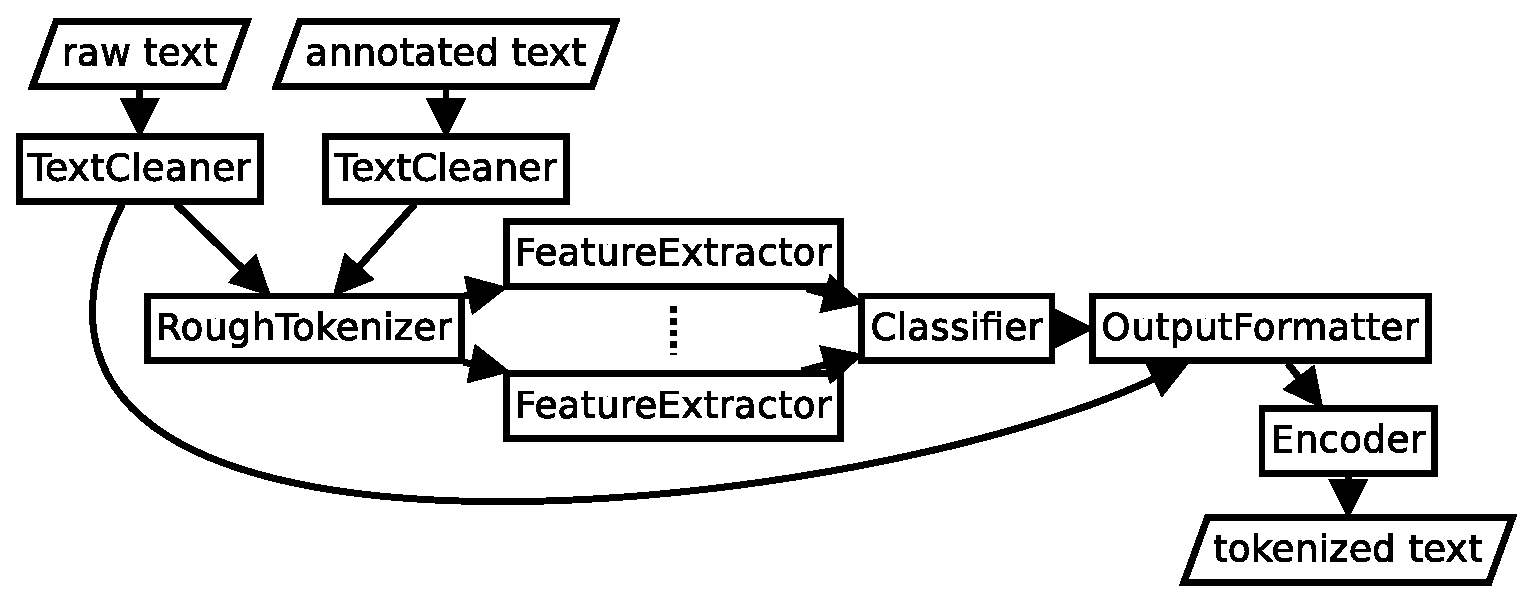
\includegraphics[width=\textwidth]{img/all-parts.eps}
  \caption{Data flow in the entire system}
  \label{fig:all-parts}
\end{figure}

\subsection{TextCleaner}

Any input which is read by the tokenizer is first processed with the
TextCleaner. This unit is responsible for decoding the stream of text and
optionally removing XML markup and expanding HTML entities and character
references. These changes to the input stream (referred to as cutouts in the
program) are conveyed to the OutputFormatter so that they can be undone in the
output. This allows the tokenizer to process XML marked up content as if it was
plaintext. The XML markup thus cannot be broken by and does not interfere with
the tokenization process.

\subsection{RoughTokenizer}

The RoughTokenizer's goal is to examine the cleaned input stream and identify
both unambiguous and ambiguous token and sentence boundaries. It does so by
splitting the text into what we call rough tokens. In the simplest case, rough
tokens are the whitespace delimited words of the text (the term word will be
used to mean a maximal subsequence of nonwhite characters). However, the user
can write regular expressions to define certain points within and between these
strings of nonwhite characters which may split them up into what end up being
the rough tokens. These user-defined points are called decision points and they
represent the ambiguous token/sentence boundaries.

There are three types of decision points. There is the MAY\_SPLIT which occurs
within words and signals a potential token boundary. The MAY\_BREAK\_SENTENCE
occurs before and after certain characters and marks a potential sentence
boundary. MAY\_SPLIT and MAY\_BREAK\_SENTENCE are the decision points which
split words into rough tokens. The third type of decision point is MAY\_JOIN
which occurs between words and turns the space between them from a token
boundary to a potential token boundary, making it possible for the two words to
join into a single token.

The rough tokenizer detects all decision points in the text and produces a
stream of discrete rough tokens annotated with information about surrounding
whitespace and decision points.

\subsection{FeatureExtractor}



\chapter{User Documentation}
\label{chap:userdoc}

In this chapter we go over the specific way the user sets up the tokenizer 

\chapter{Evaluation}
\label{chap:eval}

\chapter*{Conclusion}
\addcontentsline{toc}{chapter}{Conclusion}

We have presented a data-driven system for tokenizing and segmenting text. We
have demonstrated the system's versatility by combining methods based on
different techniques such as morphological dictionaries, regular expressions
and exception lists. The system proved its universal applicability in being
able to act both as a sentence boundary disambiguator for languages such as
English and Czech and as a word segmenter for languages which do not use
whitespace such as Chinese. We have also pointed to the fact that the program
relies only on multiplatform programs and libraries. While it has not been
tested on Windows or MacOS yet, care was taken at every step to ensure it would
be a smooth transition (ICU can be used instead of libiconv for character code
conversion, CMake is used for building, OS-specific matters are accessed via
Boost only\ldots).

We measured the accuracy, precision, recall and F-measure of the token and
sentence boundary disambiguation. The tests were executed with several very
different tokenization schemes and on several datasets in multiple languages.
We also measured and analyzed the tokenizer's speed and identified the
bottleneck which should serve as an avenue for further optimization.

The natural next step would be to invent and experiment with new ways and
features for tokenizing and segmenting text. The system offers fast feedback on
the accuracy of the user's tokenization schemes and is helpful in pointing out
positions in the text which are yet to be covered by rules for inserting
decision points. Another possible elaboration might be to change the maximum
entropy training backend to the Toolkit for Advanced Discriminative Modelling
or some other alternative.


\appendix
\chapter{Automatic Detection of Irregular Annotation}
\label{chap:irreg}


%%% Seznam použité literatury
%%% Seznam použité literatury je zpracován podle platných standardů. Povinnou citační
%%% normou pro bakalářskou práci je ISO 690. Jména časopisů lze uvádět zkráceně, ale jen
%%% v kodifikované podobě. Všechny použité zdroje a prameny musí být řádně citovány.

\def\bibname{Bibliography}
\begin{thebibliography}{99}
\addcontentsline{toc}{chapter}{\bibname}

%\bibitem{lamport94}
%  {\sc Lamport,} Leslie.
%  \emph{\LaTeX: A Document Preparation System}.
%  2. vydání.
%  Massachusetts: Addison Wesley, 1994.
%  ISBN 0-201-52983-1.

\bibitem{lamport94}
  {\sc Lamport,} Leslie.
  \emph{\LaTeX: A Document Preparation System}.
  2. vydání.
  Massachusetts: Addison Wesley, 1994.
  ISBN 0-201-52983-1.

\bibitem{mxterm}
  {\sc Reynar,} Jeffrey C. and Ratnaparkhi, Adwait.
  \emph{A maximum entropy approach to identifying sentence boundaries.}
  1997. In Proceedings of the fifth conference on
Applied natural language processing (ANLC '97). Association for Computational
Linguistics, Stroudsburg, PA, USA, 16-19. DOI=10.3115/974557.974561
http://dx.doi.org/10.3115/974557.974561\end{thebibliography}


%%% Tabulky v bakalářské práci, existují-li.
\chapwithtoc{List of Tables}

%%% Použité zkratky v bakalářské práci, existují-li, včetně jejich vysvětlení.
\chapwithtoc{List of Abbreviations}

%%% Přílohy k bakalářské práci, existují-li (různé dodatky jako výpisy
%%% programů, diagramy apod.). Každá příloha musí být alespoň jednou
%%% odkazována z vlastního textu práce. Přílohy se číslují.
\chapwithtoc{Attachments}

\openright
\end{document}
